\section{GUI plotting performance}
    We evaluated the performance of the GUI plotting routine. We evaluated the routine when plotting the sampling window observed $\Delta$Q, the mean and confidence bounds of the polling window of observed $\Delta$Qs. The procedure is the same for an observed and calculated $\Delta$Q, so we would need to double the results we have to obtain the total time for the plot
    The routine first prepares the $\Delta$Qs, creating vectors of QPointF (a Qt class representing a point for a QtChart), representing all the x and y values of the $\Delta$Qs CDF. The vectors are created for the lower bound, the upper bound, the mean of the window of $\Delta$Qs and the observed $\Delta$Q.

    Then, once the vectors are prepared, Qt replaces the old points with the new points for every series being plotted.

    \begin{figure}[H]
        \begin{center}
            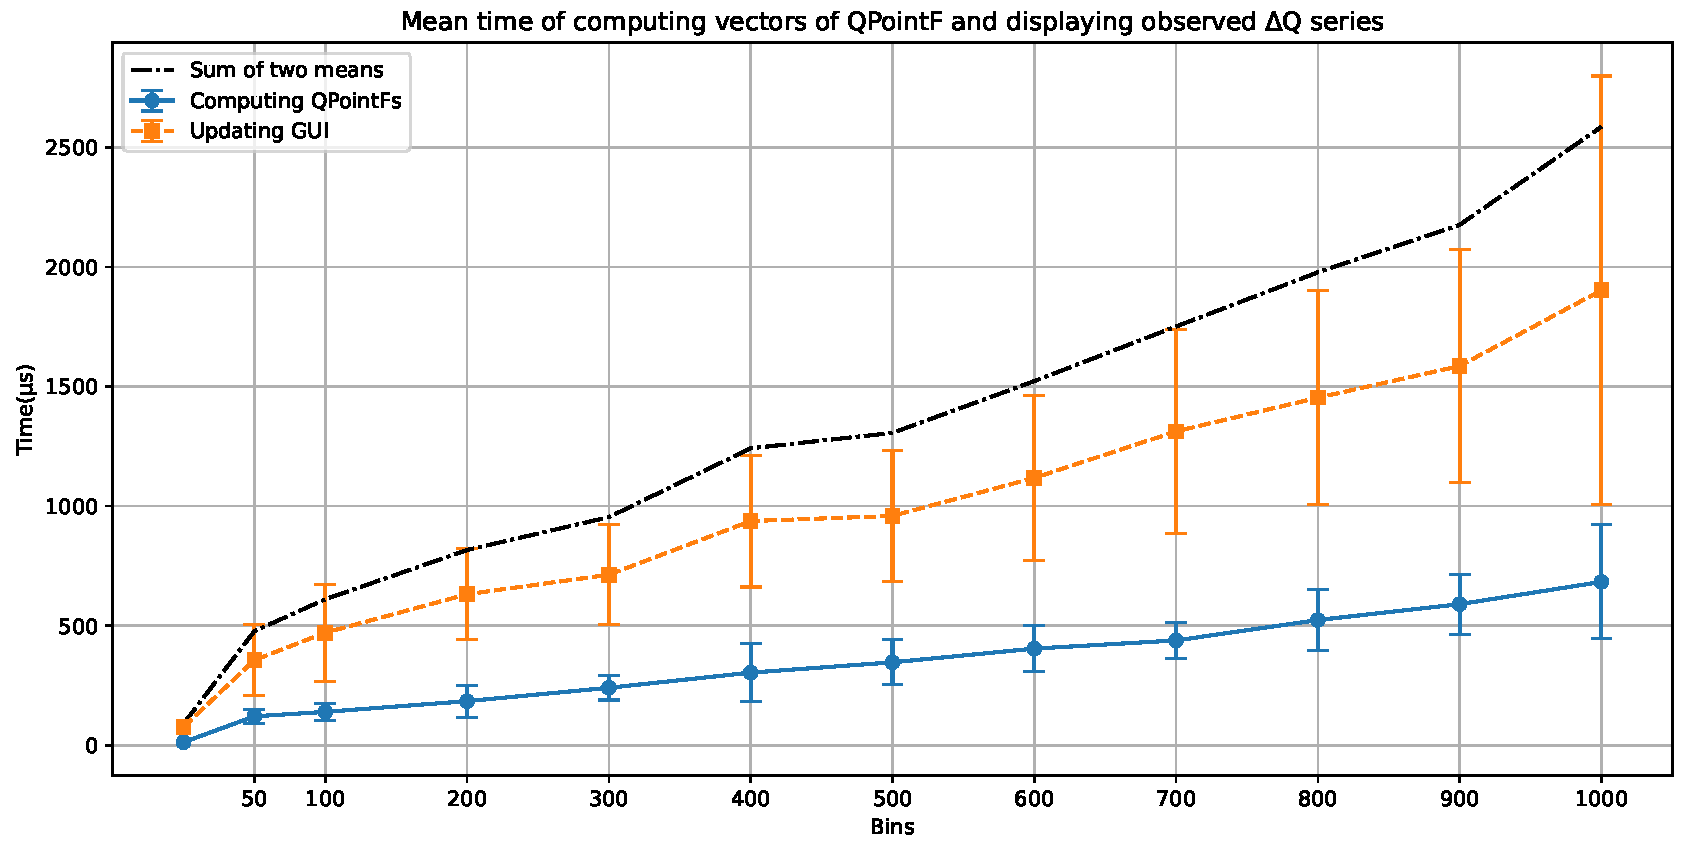
\includegraphics[width = 0.85\textwidth]{img/plots.pdf}
        \end{center}
        \caption{Performance of plotting sampling window and polling window observable $\Delta$Q. \textbf{(Blue, circle)}: QPoinfF vectors setup performance. \textbf{(Orange, square)}: Plotting performance. \textbf{(Black, dotted)}: Sum of the previous two.}
    \end{figure}
    
    The result scales up to 2 ms for 1000 bins. We believe that these performances are the choke point of the oscilloscope. If we were to plot the calculated $\Delta$Q and its confidence bounds, the time increase would be twofold. If the sampling rate was 100ms, some frames would probably be skipped if the number of bins = 1000. The results may nevertheless be explained by the specifications of the PC where we ran the tests, namely by the CPU and the GPU (\cref{app:pc_spec}).
